\documentclass[11pt,a4paper]{article}
\usepackage[utf8]{inputenc}
\usepackage[T1]{fontenc}
\usepackage[spanish,es-tabla,es-noshorthands]{babel}
\usepackage[a4paper,top=3.8cm,bottom=2.8cm,left=2cm,right=2cm,headheight=2.3cm,headsep=0.35cm,footskip=1.25cm]{geometry}
\usepackage[scaled=0.95]{helvet}
\renewcommand{\familydefault}{\sfdefault}
\usepackage{microtype}
\usepackage{array}
\usepackage{multirow}
\usepackage{tabularx}
\usepackage{longtable}
\usepackage{booktabs}
\usepackage{xcolor}
\usepackage{colortbl}
\usepackage{enumitem}
\usepackage{caption}
\usepackage{graphicx}
\usepackage{placeins}
\usepackage{lastpage}
\usepackage{fancyhdr}
\usepackage{eso-pic}
\usepackage{tikz}
\usepackage{tocloft}
\usepackage[hidelinks]{hyperref}

\newcolumntype{L}[1]{>{\raggedright\arraybackslash}p{#1}}
\newcolumntype{Y}{>{\raggedright\arraybackslash}X}
\captionsetup{font=small,labelfont=bf}
\setlist{itemsep=2pt,topsep=3pt}
\setlength{\parskip}{0.3em}
\setlength{\emergencystretch}{1.5em}

\definecolor{hdrgray}{gray}{0.85}

% indice: leaders punteados tambien en secciones
\renewcommand{\cftsecleader}{\cftdotfill{\cftdotsep}}
\renewcommand{\cftsecfont}{\bfseries}
\renewcommand{\cftsecpagefont}{\normalfont}
\setlength{\cftbeforesecskip}{4pt}

% caja de encabezado (cada pagina), a lo ancho del cuerpo
\newcommand{\encabezado}{\scriptsize
\setlength{\tabcolsep}{3pt}%
\begin{tabularx}{\textwidth}{|>{\centering\arraybackslash}m{4.6cm}|>{\centering\arraybackslash}X|>{\centering\arraybackslash}m{3.2cm}|}
\hline
\bfseries Pontificia Universidad Javeriana &
PROCESO\newline Ciclo de Desarrollo de Software\newline Documento: Plan de Pruebas &
Ingeniería en Sistemas\\
\hline
\end{tabularx}}

% caja de pie (cada pagina), a lo ancho del cuerpo
\newcommand{\piedepagina}{\scriptsize
\setlength{\tabcolsep}{3pt}%
\begin{tabularx}{\textwidth}{|m{4.6cm}|>{\centering\arraybackslash}X|>{\raggedleft\arraybackslash}m{3.2cm}|}
\hline
Joshua Mendez\newline Edinson Pedroza &
\begin{tabular}{@{}c@{}}Pontificia Universidad Javeriana\\ Ingeniería en Sistemas\end{tabular} &
Fecha: \today\newline Página \thepage{} de \pageref{LastPage}\\
\hline
\end{tabularx}}

\fancypagestyle{plantilla}{%
  \fancyhf{}%
  \renewcommand{\headrulewidth}{0pt}%
  \renewcommand{\footrulewidth}{0pt}%
  \fancyhead[C]{\encabezado}%
  \fancyfoot[C]{\piedepagina}%
}
% que el estilo "plain" (portada, índice) también use la plantilla
\fancypagestyle{plain}{%
  \fancyhf{}%
  \renewcommand{\headrulewidth}{0pt}%
  \renewcommand{\footrulewidth}{0pt}%
  \fancyhead[C]{\encabezado}%
  \fancyfoot[C]{\piedepagina}%
}

% borde de pagina alrededor del cuerpo
\AddToShipoutPictureBG{%
 \begin{tikzpicture}[remember picture,overlay]
  \draw[line width=0.5pt]
    ([xshift=2cm,yshift=2.35cm]current page.south west) rectangle
    ([xshift=-2cm,yshift=-3.6cm]current page.north east);
 \end{tikzpicture}}

\pagestyle{plantilla}

\begin{document}
\thispagestyle{plantilla}

% -------- PORTADA --------
\vspace*{5.5cm}
\begin{center}
{\fontsize{26}{30}\selectfont\bfseries PLAN DE PRUEBAS}\\[0.5cm]
{\large Sistema bajo prueba: Demoblaze, tienda en línea de demostración}\\[1.6cm]
{\large\bfseries VERSIÓN 1.0}\\[2.5cm]
{\normalsize Joshua Mendez}\\[0.15cm]
{\normalsize Edinson Pedroza}\\[0.25cm]
{\normalsize Construcción de Software y Pruebas \quad Grupo A \quad 2026-2}\\[0.25cm]
{\normalsize Profesora: Claudia Martínez}
\end{center}
\clearpage

% -------- HOJA RESUMEN DE MODIFICACIONES --------
\phantomsection\addcontentsline{toc}{section}{Hoja resumen de modificaciones}
\vspace*{0.8cm}
\begin{center}\underline{\textbf{\large HOJA RESUMEN DE MODIFICACIONES}}\end{center}
\vspace{0.6cm}
{\small
\renewcommand{\arraystretch}{1.5}
\noindent\begin{tabularx}{\textwidth}{|c|c|Y|L{2.7cm}|L{2.7cm}|}
\hline
\rowcolor{black}
\textcolor{white}{\textbf{Versión}} & \textcolor{white}{\textbf{Fecha}} & \textcolor{white}{\textbf{Cambios respecto de la versión anterior}} & \textcolor{white}{\textbf{Preparado por}} & \textcolor{white}{\textbf{Aprobado por}}\\
\hline
1.0 & \today & Versión inicial & Joshua Mendez\newline Edinson Pedroza & Claudia Martínez\\
\hline
\end{tabularx}}
\clearpage

% -------- ÍNDICE --------
\renewcommand{\contentsname}{ÍNDICE}
\renewcommand{\cfttoctitlefont}{\hfill\large\bfseries}
\renewcommand{\cftaftertoctitle}{\hfill}
\tableofcontents
\clearpage



%------------------------------------------------------------------
\FloatBarrier
\section*{Sistema bajo prueba y nota preliminar}
\phantomsection\addcontentsline{toc}{section}{Sistema bajo prueba y nota preliminar}

Este plan cubre \textbf{Demoblaze} (\url{https://www.demoblaze.com}), una tienda en
línea de demostración publicada por BlazeMeter, que es uno de los sitios propuestos
por la docente para el ejercicio.

Trabajamos en grupo: Joshua Mendez y Edinson Pedroza. El reparto de funciones entre
los dos está en la sección de roles.

Algo importante antes de empezar: el sistema no es nuestro. No tengo el código fuente,
ni entro al servidor, ni veo la base de datos o los logs, y tampoco puedo pedir que
arreglen un defecto. Eso cambia para qué sirve este plan. No estamos certificando un
producto antes de sacarlo a producción, porque ya está en producción. Lo que hacemos es
medir la calidad que se puede ver desde afuera y dejar anotado lo que encontremos.
Por eso hay varios criterios típicos de un plan de pruebas que tuvimos que adaptar, y
lo avisamos en cada sección donde pasa.

El documento sigue las ocho secciones que pide el taller. Para armarlas nos apoyamos en
Katalon (s.f.), y para los nombres de niveles y tipos en Martínez (2026a, 2026b) e
ISTQB (2018).

%------------------------------------------------------------------
\FloatBarrier
\section*{1. Alcance}
\phantomsection\addcontentsline{toc}{section}{1. Alcance}

\subsection*{1.1 Dentro del alcance}
\addcontentsline{toc}{subsection}{1.1 Dentro del alcance}

Recorrimos el sitio entero y revisamos sus elementos para listar todo lo que el usuario
puede hacer. La tabla cubre todas las funciones que cambian algo en el sistema. Lo
que es solo presentación y no cambia nada, como el carrusel de la portada, el pie de
página y el video de About us, lo dejamos junto en la última fila y de eso solo revisamos
que cargue bien.

\begingroup
\small
\renewcommand{\arraystretch}{1.2}
\begin{table}[htb]\centering\small
\caption{Funcionalidad incluida en el alcance.}\label{tab:alcance}
\begin{tabularx}{\textwidth}{@{}L{3.6cm} Y@{}}
\toprule
\textbf{Módulo} & \textbf{Qué se prueba} \\
\midrule
Catálogo & Listado de productos en la página principal, filtrado por las tres categorías (Phones, Laptops, Monitors), paginación, y consistencia entre el precio del listado y el del detalle. \\
Detalle de producto & Carga de la ficha por identificador, datos mostrados (nombre, precio, descripción, imagen) y acción de agregar al carrito. \\
Carrito & Agregar uno y varios productos, eliminar, cálculo del total, persistencia del contenido al navegar entre páginas. \\
Registro (Sign up) & Alta de usuario con datos válidos, usuario duplicado, campos vacíos y límites de longitud. \\
Autenticación (Log in) & Ingreso con credenciales válidas e inválidas, campos vacíos, y cierre de sesión. \\
Orden de compra & Formulario de compra, con el total precargado y sus seis campos editables (nombre, país, ciudad, tarjeta, mes, año): validaciones, confirmación y contenido del comprobante. \\
Contacto & Envío del formulario con datos válidos e inválidos y comportamiento con campos vacíos. \\
Interfaz y accesibilidad & Asociación de etiquetas con campos en los formularios, navegación por teclado y comportamiento responsivo básico. \\
Elementos de presentación & Carga sin error del carrusel de la portada, del pie de página y del reproductor de la ventana About us. No se verifica su contenido. \\
Rendimiento & Métricas web esenciales de la página principal contra los umbrales publicados por Google, medidas sobre usuarios reales en escritorio y en móvil. Diseño de las pruebas de carga y de estrés con su perfil, herramienta y umbrales. \\
Integración entre sistema y producto & Contrato entre la interfaz y el servicio HTTP que consume: códigos de respuesta, forma de los datos, consistencia entre respuestas y manejo de errores en la interfaz. \\
Seguridad & Cabeceras de seguridad de la respuesta, manejo de la contraseña en el login, enumeración de usuarios, inyección en el login y política CORS de la API. No incluye denegación de servicio. \\
Compatibilidad de navegadores & Que la tienda cargue y se vea bien en los tres motores de navegador que existen (Blink, Gecko y WebKit), en escritorio y en móvil. La matriz por riesgo y lo cubierto van en el apartado 3.12. \\
\bottomrule
\end{tabularx}
\end{table}
\endgroup

\subsection*{1.2 Fuera del alcance}
\addcontentsline{toc}{subsection}{1.2 Fuera del alcance}

\begin{itemize}
  \item \textbf{Pruebas de componente.} Requieren acceso al código fuente
        (Martínez, 2026a) y no lo hay.
  \item \textbf{Pruebas de integración entre componentes.} Esas sí necesitan el
        código y quedan fuera. La integración entre sistema y producto, en cambio,
        sí entra: está en el apartado 3.9 con los resultados.
  \item \textbf{Pruebas de denegación de servicio.} Inundar el sitio con tráfico
        afectaría a las demás personas que lo usan, así que quedan fuera. El resto
        de pruebas de seguridad sí entra, y están en el apartado 3.11 con los
        resultados.
  \item \textbf{El reproductor de video de la ventana About us}, más allá de
        comprobar que la ventana abre y el reproductor carga.
  \item \textbf{Persistencia de datos a largo plazo.} El sitio de demostración se
        reinicia cada tanto y nadie garantiza que los datos se queden. Probar que un
        usuario creado hoy siga ahí la otra semana no diría nada útil.
  \item \textbf{Automatización de la ejecución.} Esta iteración es manual. En la
        sección 3 indico qué se automatizaría y por qué no se hace ahora.
\end{itemize}

%------------------------------------------------------------------
\FloatBarrier
\section*{2. Criterios de entrada y salida (DoR y DoD)}
\phantomsection\addcontentsline{toc}{section}{2. Criterios de entrada y salida (DoR y DoD)}

Uso el DoR para las condiciones que se tienen que cumplir antes de empezar a
probar, y el DoD para las que permiten decir que las pruebas ya terminaron. Partí de
las listas de entrada y salida de Katalon (s.f.) y las ajustamos a un sistema que no
controlo.

\subsection*{2.1 Definition of Ready: criterios de entrada}
\addcontentsline{toc}{subsection}{2.1 Definition of Ready: criterios de entrada}

\begin{enumerate}[label=E\arabic*.]
  \item Este plan está revisado y aprobado.
  \item Los casos de prueba están escritos, con resultado esperado explícito, y
        revisados antes de ejecutarse.
  \item Una prueba rápida de sanidad sale bien: carga la página principal, abre la
        ficha de un producto y abre el carrito. Si esto falla, ni empiezo, porque
        los resultados no dirían nada del software sino de que el sitio está
        caído.
  \item El navegador de referencia está instalado y su versión queda registrada.
  \item Los datos de prueba están definidos: usuario y contraseña ficticios,
        número de tarjeta ficticio y valores de borde para cada campo.
  \item Existe una plantilla de registro de ejecución y otra de reporte de
        defectos.
\end{enumerate}

\subsection*{2.2 Definition of Done: criterios de salida}
\addcontentsline{toc}{subsection}{2.2 Definition of Done: criterios de salida}

\begin{enumerate}[label=S\arabic*.]
  \item El 100\,\% de los casos de prioridad alta está ejecutado, y al menos el
        80\,\% del total.
  \item Al menos el 90\,\% de los casos ejecutados resulta aprobado. Tomo este
        umbral del documento de ejemplo entregado con el taller, que fija una
        aceptación del 90\,\% sobre el total ejecutado.
  \item Todo defecto encontrado está registrado con pasos de reproducción,
        evidencia gráfica y severidad asignada según la clasificación de la
        sección 7.
  \item Los casos que fallaron por una causa ajena al software, como una caída del
        sitio, están reejecutados o marcados como no concluyentes con su
        justificación.
  \item El informe de resumen de pruebas está entregado, con las métricas de la
        sección 4.
\end{enumerate}

%------------------------------------------------------------------
\FloatBarrier
\section*{3. Estrategia de pruebas}
\phantomsection\addcontentsline{toc}{section}{3. Estrategia de pruebas}

Antes de entrar, una aclaración de nombres. Katalon (s.f.) dedica todo su artículo a
separar el plan de pruebas de la estrategia de pruebas. El plan es de un proyecto
puntual; la estrategia es algo más general, de toda una organización. Así que lo que
va en esta sección no es una estrategia de empresa sino cómo pensamos probar este
sitio en concreto.

\subsection*{3.1 Niveles y tipos}
\addcontentsline{toc}{subsection}{3.1 Niveles y tipos}

Como no tengo el código, las pruebas de componente no van. El grueso del trabajo se
hace en el nivel de sistema, revisando el producto de punta a punta como lo vería un
usuario (Martínez, 2026a). La integración entre sistema y producto sí se puede
probar por caja negra, y la desarrollo en el apartado 3.9.

Casi todos los casos son funcionales. Hay una parte menor de usabilidad,
accesibilidad y rendimiento, que es no funcional (Martínez, 2026b).

\subsection*{3.2 Técnicas de diseño de casos}
\addcontentsline{toc}{subsection}{3.2 Técnicas de diseño de casos}

\begin{itemize}
  \item \textbf{Partición de equivalencias} en los campos de texto de los cuatro
        formularios, separando entradas válidas, inválidas y vacías.
  \item \textbf{Análisis de valores límite} en la longitud de usuario y
        contraseña, y en los campos de mes y año del formulario de compra, que son
        los únicos dominios ordenados con un borde definido.
  \item \textbf{Transición de estados} para el ciclo del carrito: vacío, con un
        producto, con varios, tras agregar dos veces el mismo, tras eliminar y tras
        completar la compra.
  \item \textbf{Tabla de decisión} para la compra, desarrollada en el apartado
        siguiente.
\end{itemize}

No todos los casos salen de una técnica de diseño. Algunos son revisiones de
consistencia, como comparar el comprobante con el total del carrito, y otros son
inspecciones, como mirar si las etiquetas de los formularios apuntan al campo que
toca.

\subsection*{3.3 Tabla de decisión de la compra}
\addcontentsline{toc}{subsection}{3.3 Tabla de decisión de la compra}

La compra depende de tres condiciones de sí o no, así que salen ocho combinaciones.
La tabla las muestra todas, marca cuáles voy a probar y dice por qué dejo las otras
por fuera.

\begingroup
\footnotesize
\setlength{\tabcolsep}{4pt}
\renewcommand{\arraystretch}{1.2}
\begin{table}[htb]\centering\footnotesize
\caption{Tabla de decisión del formulario de compra.}\label{tab:decision}
\begin{tabularx}{\textwidth}{@{}c c c c L{3.4cm} Y@{}}
\toprule
\textbf{\#} & \textbf{Sesión} & \textbf{Carrito} & \textbf{Campos} & \textbf{Resultado esperado} & \textbf{Caso} \\
\midrule
1 & Sí & Con productos & Completos & Compra exitosa con comprobante & CP-COM-01 \\
2 & Sí & Con productos & Incompletos & Rechazo por campos obligatorios & CP-COM-04 \\
3 & Sí & Vacío & Completos & Rechazo por carrito vacío & CP-COM-02 \\
4 & No & Con productos & Completos & Se exige iniciar sesión & CP-COM-03 \\
5 & Sí & Vacío & Incompletos & Rechazo & Descartada \\
6 & No & Con productos & Incompletos & Rechazo & Descartada \\
7 & No & Vacío & Completos & Rechazo & Descartada \\
8 & No & Vacío & Incompletos & Rechazo & Descartada \\
\bottomrule
\end{tabularx}
\end{table}
\endgroup

Las combinaciones 5 a 8 las descartamos porque cada una junta dos o tres motivos de
rechazo que ya revisamos por separado en la 2, la 3 y la 4. No nos dirían nada nuevo, y
si el sistema fallara sería más difícil saber cuál de los motivos lo causó.

\subsection*{3.4 Criterios de referencia}
\addcontentsline{toc}{subsection}{3.4 Criterios de referencia}

El resultado esperado de cada caso se fija contra estándares públicos, no contra un
criterio propio: comparo el sitio con lo que se le exige a cualquier software.

\textbf{Modelo de calidad.} La norma ISO/IEC 25010 lista ocho características de
calidad: adecuación funcional, eficiencia de desempeño, compatibilidad, usabilidad,
fiabilidad, seguridad, mantenibilidad y portabilidad. De esas ocho puedo mirar cinco
desde afuera: adecuación funcional, eficiencia de desempeño, compatibilidad,
usabilidad y fiabilidad. Mantenibilidad y portabilidad necesitan el código, y
seguridad queda fuera por lo que ya expliqué en el alcance. Cada módulo de la
Tabla 1 lo pruebo contra la característica que le toca.

\textbf{Accesibilidad.} Aquí el criterio son las WCAG 2.1 del W3C. El hallazgo del
apartado 3.8, donde las etiquetas de los formularios no apuntan a sus campos, rompe
dos criterios de nivel A: el 1.3.1, información y relaciones, y el 4.1.2, nombre,
función y valor.

\textbf{Rendimiento.} Google publica umbrales concretos para las métricas web
esenciales y son los que uso en el apartado 3.10: Largest Contentful Paint de máximo
2,5 segundos, Interaction to Next Paint de máximo 200 milisegundos y Cumulative
Layout Shift de máximo 0,10.

\textbf{Convenciones del dominio.} Cuando no hay estándar que aplique, el criterio
es lo que cualquiera espera de una tienda en línea: que no deje comprar con el
carrito vacío, que el total dé igual a la suma de lo que muestra, que el precio del
listado sea el mismo del detalle y que un error de login no deje adivinar si el
usuario existe. Son expectativas comunes a cualquier comercio electrónico.

En la suite, cada caso indica en una columna cuál de estos cuatro criterios se le
aplica.

\subsection*{3.5 Pruebas asociadas al cambio}
\addcontentsline{toc}{subsection}{3.5 Pruebas asociadas al cambio}

Yo no despliego nada, pero el sitio puede cambiar de un día para otro sin avisar.
Por eso dejo armada desde ya una regresión mínima: el flujo de compra completo más
el registro y el inicio de sesión. Si noto que algo cambió durante las pruebas, la
vuelvo a correr. La prueba de confirmación queda definida por si llegan a arreglar
algún defecto.

\subsection*{3.6 Priorización}
\addcontentsline{toc}{subsection}{3.6 Priorización}

Ordeno el trabajo por riesgo y no por lo que sea más cómodo. Primero el flujo de
compra, que es para lo que existe una tienda y donde una falla pega más fuerte.
Después login y registro, porque de ellos depende poder comprar. Al final catálogo,
contacto y los temas de interfaz.

\subsection*{3.7 Ejecución manual, y qué se automatizaría}
\addcontentsline{toc}{subsection}{3.7 Ejecución manual, y qué se automatizaría}

Esta vuelta la hacemos manual, porque con esta cantidad de casos todavía no se
justifica automatizar. Si el ejercicio siguiera, automatizaría
la regresión del apartado 3.5, que es la que se repite. Un detalle a tener en
cuenta: el sitio confirma varias acciones con diálogos de JavaScript, y esos
diálogos frenan la automatización si la herramienta no está preparada para
manejarlos. Eso habría que resolverlo antes.

\subsection*{3.8 Hallazgo de la exploración preliminar}
\addcontentsline{toc}{subsection}{3.8 Hallazgo de la exploración preliminar}

Mientras reconocíamos el sitio, revisando el árbol de accesibilidad nos dimos cuenta de que
en los formularios \emph{Place order} y \emph{Contact} las etiquetas no están bien
asociadas a sus campos. El campo que va después de \emph{Name} se anuncia como
\emph{Total}, y el que va después de \emph{Contact Name} se anuncia como
\emph{Contact Email}. Un lector de pantalla leería un nombre que no es el del campo.
Por eso incluí la accesibilidad en el alcance.

\subsection*{3.9 Integración entre sistema y producto: resultados}
\addcontentsline{toc}{subsection}{3.9 Integración entre sistema y producto: resultados}

La interfaz de Demoblaze no calcula nada por su cuenta: todo se lo pide a un servicio
HTTP aparte, en \texttt{api.demoblaze.com}. Esa unión sí la puedo probar por caja
negra, mirando el tráfico del navegador y llamando al servicio directo. Corrí cuatro
casos y encontré tres problemas.

\begingroup
\footnotesize
\setlength{\tabcolsep}{4pt}
\renewcommand{\arraystretch}{1.2}
\begin{table}[htb]\centering\footnotesize
\caption{Resultados de las pruebas de integración entre la interfaz y su servicio.}
\begin{tabularx}{\textwidth}{@{}L{1.6cm} L{3.0cm} Y L{1.7cm}@{}}
\toprule
\textbf{Caso} & \textbf{Llamada} & \textbf{Resultado observado} & \textbf{Estado} \\
\midrule
CP-ISP-01 & \texttt{GET /entries} & Responde 200 en 0,44 s con 9 productos. La portada muestra esos mismos 9. & Aprobado \\
CP-ISP-02 & \texttt{POST /bycat} & Responde 200 con preflight CORS. Devuelve 7 teléfonos, 6 portátiles y 2 monitores, o sea 15 productos. Pero \texttt{/entries} solo devuelve 9. Los dos servicios pagina distinto y la portada nunca muestra 6 de los 15 productos hasta que uno pasa de página. & Fallido \\
CP-ISP-03 & \texttt{POST /view} & Responde 200 y el título y el precio coinciden con lo que trae \texttt{/entries} para el mismo id. & Aprobado \\
CP-ISP-04 & \texttt{POST /view} con id inexistente & Responde \textbf{200 OK} con el cuerpo \texttt{\{"errorMessage":"Not found."\}}. Debería responder 404. La interfaz no revisa ese caso y pinta \emph{undefined} en título, precio y descripción, con el botón de agregar al carrito funcionando. & Fallido \\
\bottomrule
\end{tabularx}
\end{table}
\endgroup

\begin{figure}[htb]\centering

\includegraphics[width=0.95\textwidth]{defecto-producto-inexistente.png}
\caption{Página de producto con un identificador que no existe. El servicio responde 200 y la interfaz muestra \emph{undefined}.}
\end{figure}

El CP-ISP-04 es el más serio de los tres, y es porque junta dos errores. El servicio
miente con el código de estado, y la interfaz le cree sin mirar el cuerpo de la
respuesta. Un cliente que valide solo por el código, que es lo normal, tomaría un
producto inexistente como si existiera. También lo probamos desde la interfaz: al darle
a agregar al carrito sobre ese producto fantasma, el sitio responde ``Product
added'' y el carrito queda vacío. Me confirmó una acción que en realidad no pasó.

Ya que estaba mirando el tráfico, vi otra cosa: el video de la ventana About us se
descarga en todas las páginas, incluida la ficha de producto, aunque la ventana esté
cerrada y el video no se vea nunca. Son segmentos \texttt{.ts} que se bajan sin que
nadie los pida, y eso ayuda a explicar los tiempos del apartado siguiente.

\subsection*{3.10 Rendimiento, carga y estrés}
\addcontentsline{toc}{subsection}{3.10 Rendimiento, carga y estrés}

\textbf{Lo que sí medí.} Medí la página principal con una herramienta pública de análisis de rendimiento web,
que muestra las métricas tomadas de usuarios reales de Chrome en los últimos 28
días. La Figura 1 es la captura de esa medición.

\begin{figure}[htb]\centering
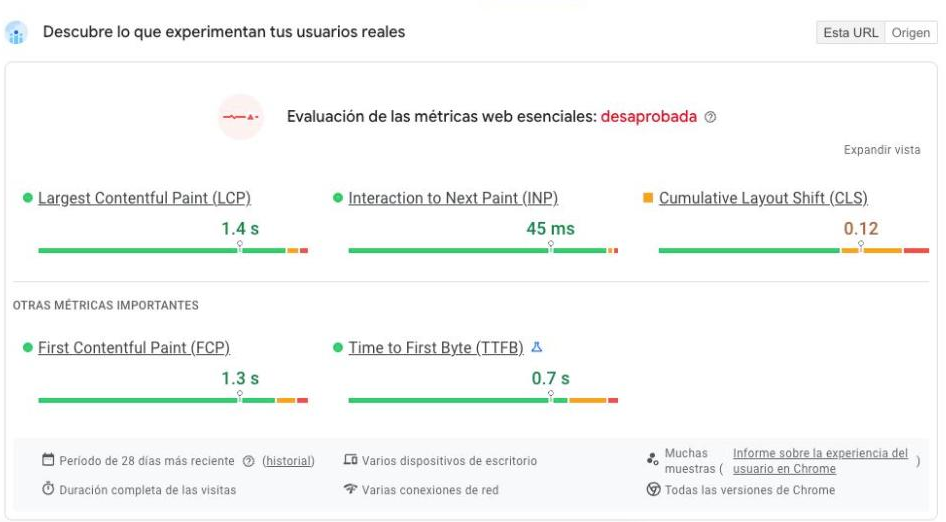
\includegraphics[width=0.92\textwidth]{rendimiento-escritorio.png}
\caption{Métricas web esenciales de Demoblaze, medidas sobre usuarios reales el 14 de septiembre de 2026.}
\end{figure}

\begingroup
\small
\renewcommand{\arraystretch}{1.2}
\begin{table}[htb]\centering\small
\caption{Resultados de rendimiento contra los umbrales publicados por Google.}
\begin{tabularx}{\textwidth}{@{}L{5.2cm} L{2.4cm} L{2.8cm} Y@{}}
\toprule
\textbf{Métrica} & \textbf{Medido} & \textbf{Umbral bueno} & \textbf{Estado} \\
\midrule
Largest Contentful Paint (LCP) & 1,4 s & hasta 2,5 s & Cumple \\
Interaction to Next Paint (INP) & 45 ms & hasta 200 ms & Cumple \\
Cumulative Layout Shift (CLS) & 0,12 & hasta 0,10 & \textbf{No cumple} \\
First Contentful Paint (FCP) & 1,3 s & hasta 1,8 s & Cumple \\
Time to First Byte (TTFB) & 0,7 s & hasta 0,8 s & Cumple \\
\bottomrule
\end{tabularx}
\end{table}
\endgroup

En escritorio la herramienta marca el resultado global como \textbf{desaprobada}, y
por una sola métrica: el desplazamiento acumulado llega a 0,12 y el umbral es 0,10. O
sea, el contenido se mueve mientras la página carga. Cuadra con lo que se ve en el
sitio: el carrusel de la portada aparece después del resto y empuja los productos
hacia abajo.

En móvil está bastante peor, y es la vista con la que la mayoría entra a una tienda.
Ahí no falla una métrica sino tres.

\begin{figure}[htb]\centering
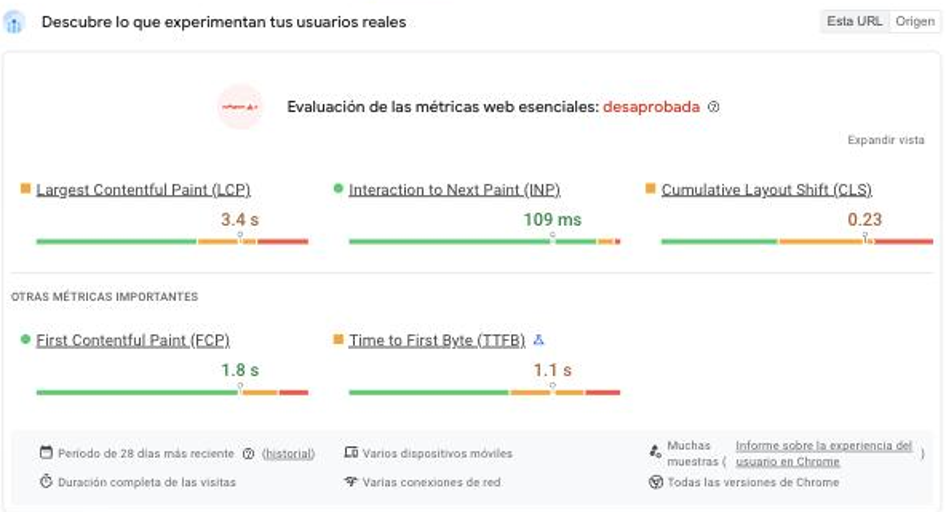
\includegraphics[width=0.92\textwidth]{rendimiento-movil.png}
\caption{Las mismas métricas medidas en móvil. Fallan LCP, CLS y TTFB.}
\end{figure}

\begingroup
\small
\renewcommand{\arraystretch}{1.2}
\begin{table}[htb]\centering\small
\caption{Comparación entre escritorio y móvil.}
\begin{tabularx}{\textwidth}{@{}L{5.0cm} L{2.0cm} L{2.0cm} L{2.4cm} Y@{}}
\toprule
\textbf{Métrica} & \textbf{Escritorio} & \textbf{Móvil} & \textbf{Umbral} & \textbf{En móvil} \\
\midrule
Largest Contentful Paint & 1,4 s & 3,4 s & hasta 2,5 s & No cumple \\
Interaction to Next Paint & 45 ms & 109 ms & hasta 200 ms & Cumple \\
Cumulative Layout Shift & 0,12 & 0,23 & hasta 0,10 & No cumple \\
First Contentful Paint & 1,3 s & 1,8 s & hasta 1,8 s & Justo en el límite \\
Time to First Byte & 0,7 s & 1,1 s & hasta 0,8 s & No cumple \\
\bottomrule
\end{tabularx}
\end{table}
\endgroup

El desplazamiento se duplica en móvil, de 0,12 a 0,23, y el tiempo hasta el primer
byte se pasa del umbral. Con lo que vi en el tráfico del apartado anterior, donde el
video se baja en todas las páginas sin que nadie lo pida, tengo una explicación
probable, aunque habría que confirmarla midiendo con el video apagado. Lo anoto como
defecto medio en móvil y leve en escritorio.

\textbf{Carga y estrés.} Estas dos las dejo diseñadas pero sin correr, por lo mismo
que las de seguridad: meterle tráfico artificial a un servidor ajeno y sin permiso
del dueño le arruinaría el sitio a los demás. El diseño de las dos pruebas es este:

\begin{itemize}
  \item \textbf{Herramienta:} una herramienta de pruebas de carga por línea de comandos, con
        reporte de percentiles.
  \item \textbf{Guion:} el flujo de compra completo, que es el crítico: abrir la
        portada, entrar a un producto, agregarlo al carrito y terminar la orden.
  \item \textbf{Prueba de carga:} subir hasta 50 usuarios concurrentes en
        5 minutos y sostenerlos 15 minutos. Umbral: percentil 95 del tiempo de
        respuesta por debajo de 3 segundos y menos del 1\,\% de errores.
  \item \textbf{Prueba de estrés:} sumar 25 usuarios cada 3 minutos hasta
        que la tasa de error pase del 5\,\% o el percentil 95 pase de los
        10 segundos. Lo que espero sacar: el punto de saturación anotado y
        evidencia de que el sistema baja de a poco en vez de caerse de golpe.
  \item \textbf{Métricas a recoger:} tiempo de respuesta por percentiles,
        transacciones por segundo, tasa de error y cuánto tarda en recuperarse al
        quitarle la carga.
\end{itemize}

\subsection*{3.11 Seguridad}
\addcontentsline{toc}{subsection}{3.11 Seguridad}

Corrí pruebas de seguridad suficientes para resolver el taller pero no para afectar
el servicio: un sondeo a nivel de la API y de las cabeceras, con seis casos. Cinco
fallaron.

\begingroup
\footnotesize
\setlength{\tabcolsep}{4pt}
\renewcommand{\arraystretch}{1.2}
\begin{table}[htb]\centering\footnotesize
\caption{Resultados de las pruebas de seguridad.}
\begin{tabularx}{\textwidth}{@{}L{1.6cm} L{3.1cm} Y L{1.6cm}@{}}
\toprule
\textbf{Caso} & \textbf{Qué se probó} & \textbf{Resultado observado} & \textbf{Estado} \\
\midrule
CP-SEG-01 & Cabeceras de seguridad de la respuesta & La página no devuelve ninguna cabecera de seguridad: falta Content-Security-Policy, Strict-Transport-Security, X-Frame-Options y X-Content-Type-Options. Eso la deja expuesta a clickjacking y a que el navegador adivine el tipo de contenido. & Fallido \\
CP-SEG-02 & Manejo de la contraseña en el login & El servicio de login recibe la contraseña como base64. Por ejemplo, \texttt{dGVzdDEyMw==} es simplemente \texttt{test123} codificado. Viaja sobre HTTPS, así que va cifrada en tránsito, pero base64 es reversible y no reemplaza a un hash. & Fallido \\
CP-SEG-03 & Enumeración de usuarios (mensaje) & Al intentar entrar con un usuario que no existe, el servicio responde con el texto exacto \texttt{User does not exist.}, distinto del que da una contraseña incorrecta. Ese mensaje deja averiguar qué nombres de usuario están registrados. & Fallido \\
CP-SEG-04 & Bypass de autenticación con inyección en el login & Tres cadenas de inyección en el usuario no lograron entrar: ninguna devolvió un token de sesión. La autenticación no se saltó. Eso sí, las tres respondieron \texttt{Wrong password.} en vez de \texttt{User does not exist.}, o sea que el servicio trató la cadena de inyección como un usuario que existe. No es un bypass, pero es una respuesta rara que valdría la pena mirar con más calma. & Aprobado \\
CP-SEG-05 & Barrido de enumeración & Los usuarios \texttt{admin}, \texttt{test} y \texttt{administrator} responden \texttt{Wrong password.}, mientras que un nombre al azar responde \texttt{User does not exist.} Queda confirmado que las cuentas existentes se pueden distinguir de las que no, una por una. & Fallido \\
CP-SEG-06 & Política CORS de la API & Ante una petición desde el origen inventado \texttt{https://sitio-atacante.example}, la API responde \texttt{Access-Control-Allow-Origin} con ese mismo origen y además \texttt{Access-Control-Allow-Credentials: true}. O sea, acepta peticiones con credenciales desde cualquier sitio web. & Fallido \\
\bottomrule
\end{tabularx}
\end{table}
\endgroup

La más grave es la configuración CORS de CP-SEG-06. Como refleja cualquier origen y a
la vez permite credenciales, deja que un sitio de terceros le haga peticiones a la
API en nombre de un usuario con la sesión abierta. Qué tanto daño haga depende de
cómo viaje la sesión, pero reflejar un origen cualquiera con las credenciales
activadas es un error de configuración que hay que arreglar. Detrás vienen la falta
de cabeceras y la enumeración de usuarios, esta última ya confirmada por los dos
lados en CP-SEG-05. La contraseña en base64 es la más leve, porque HTTPS la protege
en tránsito. La inyección en el login no logró saltarse la autenticación, aunque la
respuesta rara de CP-SEG-04 queda anotada para mirarla después.

\subsection*{3.12 Compatibilidad de navegadores}
\addcontentsline{toc}{subsection}{3.12 Compatibilidad de navegadores}

Probar todos los navegadores, versiones y dispositivos no es viable, y tampoco es lo
que se hace en la práctica: se arma una matriz por riesgo sobre lo que de verdad usa
la gente. Se simplifica porque en el mundo solo hay tres motores de navegador: Blink
(Chrome, Edge, Brave, Opera), Gecko (Firefox, Tor) y WebKit (Safari). Si la tienda
se ve bien en los tres, en escritorio y en móvil, quedan cubiertos casi todos los
usuarios.

\begingroup
\footnotesize
\setlength{\tabcolsep}{4pt}
\renewcommand{\arraystretch}{1.2}
\begin{center}\footnotesize
\captionof{table}{Matriz de compatibilidad por motor y plataforma.}
\begin{tabularx}{\textwidth}{@{}L{1.4cm} L{2.5cm} L{2.4cm} L{2.2cm} Y@{}}
\toprule
\textbf{Motor} & \textbf{Navegador} & \textbf{Plataforma} & \textbf{Estado} & \textbf{Resultado} \\
\midrule
Blink & Chrome 138 & Escritorio, Win 10 & Ejecutado & La tienda carga completa y bien maquetada. \\
Gecko & Tor Browser 14.5 & Escritorio, Win 10 & Ejecutado & Funciona. El menú superior se parte en dos líneas (DEF-14, leve). \\
Blink & Chrome Android & Móvil & Ejecutado, datos de campo & El apartado 3.10 usa datos reales de usuarios de Chrome en Android: la tienda funciona, con reparos de rendimiento (DEF-07). \\
WebKit & Safari, macOS & Escritorio & Ejecutado & La tienda se ve idéntica a Chrome: menú en una línea, carrusel con imagen y grilla de tres columnas (Figura 6). \\
WebKit & Safari, iOS & Móvil & Ejecutado & En un iPhone real. La tienda carga completa y funcional: menú, categorías, los ocho productos con imagen y el pie de página (Figura 7). \\
Blink & Tienda en iPad, 1024x768 & Tablet, layout & Ejecutado & El layout de escritorio se mantiene intacto: carrusel, grilla de tres columnas y menú en una línea. \\
Blink & Tienda en iPhone, 375x667 & Móvil, layout & Ejecutado & Las categorías y los productos se apilan bien en una columna, pero el menú no colapsa a un botón y el carrusel se ve vacío (DEF-15). \\
\bottomrule
\end{tabularx}
\end{center}
\endgroup

Para escritorio usé un servicio que abre navegadores reales en la nube. Blink y
Gecko los ejecutamos ahí (Figura 4). La única diferencia entre los dos es cosmética:
en Tor el menú se parte en dos líneas porque el navegador trae su propia fuente y
las letras quedan más anchas. El sitio se usa igual en los dos.

\begin{figure}[htb]\centering
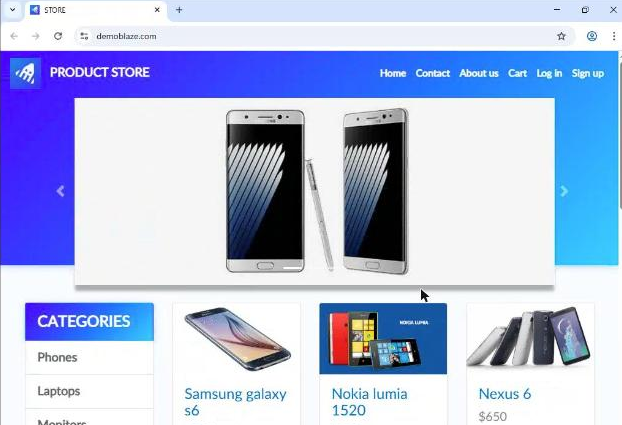
\includegraphics[width=0.49\textwidth]{compat-chrome.png}\hfill
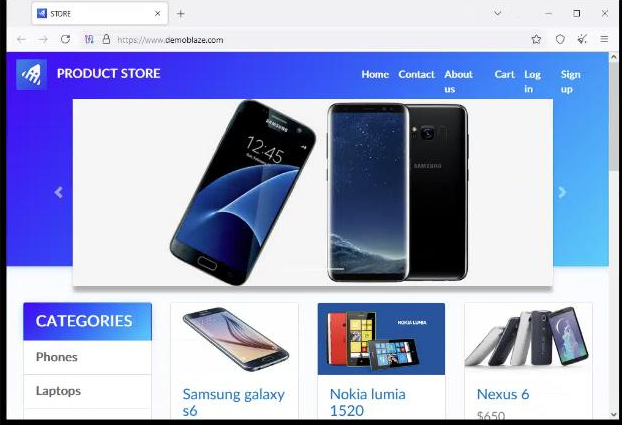
\includegraphics[width=0.49\textwidth]{compat-tor.png}
\caption{Demoblaze en Chrome, a la izquierda, y en Tor Browser, a la derecha. En el motor de Firefox los enlaces del menú superior se parten en dos líneas.}
\end{figure}

Para los distintos tamaños de pantalla usé una herramienta que carga la tienda en un
marco del tamaño de cada dispositivo, desde laptop hasta teléfono. Pude enmarcarla
justamente porque el sitio no manda la cabecera X-Frame-Options (el DEF-10 de
seguridad), así que un tercero lo puede meter en un iframe. Probé varios tamaños y
el resultado es claro: de tablet para arriba la tienda se ve igual que en
escritorio, pero en ancho de teléfono el diseño se degrada. La Figura 5 lo muestra.

\begin{figure}[htb]\centering
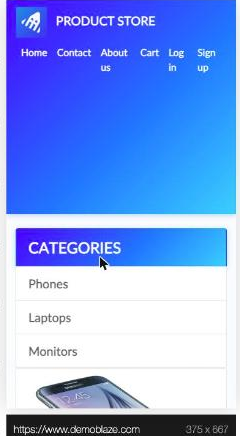
\includegraphics[height=6.2cm]{resp-movil.png}\hfill
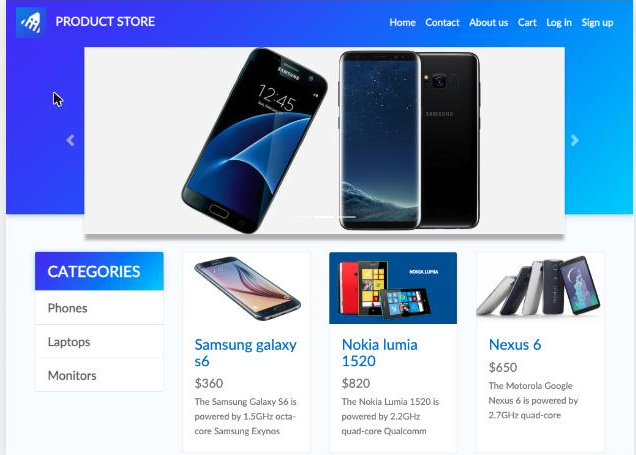
\includegraphics[height=6.2cm]{resp-tablet.png}
\caption{Demoblaze a distintos tamaños de pantalla. A la izquierda, en iPhone (375 px): el menú no colapsa a un botón y el carrusel queda vacío. A la derecha, en iPad (1024 px): el diseño de escritorio se mantiene completo.}
\end{figure}

En el teléfono la tienda sigue siendo usable, pero el menú superior se amontona en
dos filas en vez de recogerse en un botón hamburguesa, que es lo que uno esperaría
de un sitio pensado para móvil, y el carrusel de la portada aparece vacío. Lo anoto
como DEF-15, de severidad media, porque el móvil es de donde llega buena parte de
los usuarios de una tienda.

El motor WebKit en escritorio lo cerré con Safari sobre macOS. La tienda se ve igual
que en los otros dos motores, sin diferencias de maquetación (Figura 6). Con eso, los
tres motores del mundo quedan probados en escritorio, y en móvil quedan cubiertos
Blink por layout y por datos de campo (Chrome en Android).

\begin{figure}[htb]\centering
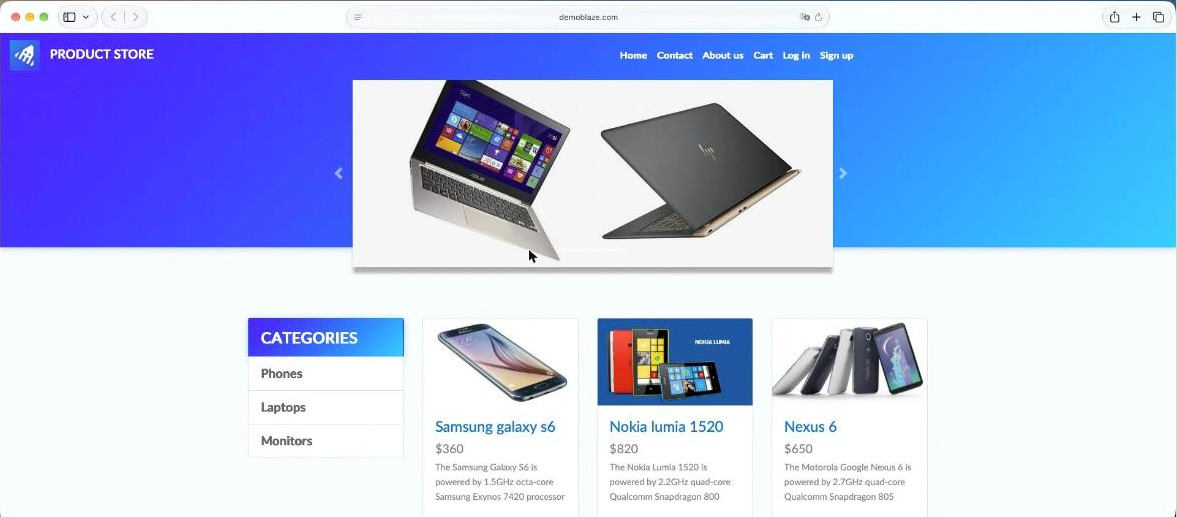
\includegraphics[width=0.85\textwidth]{compat-safari.png}
\caption{Demoblaze en Safari (motor WebKit) sobre macOS. El render es idéntico al de Chrome.}
\end{figure}

La última celda, Safari en iOS, se cerró con un iPhone real: la tienda carga
completa y se puede usar (Figura 7). Ese render viene de un guardado como PDF desde
el teléfono, que usa ancho de impresión y por eso muestra el menú en una línea y no
el layout exacto de 375 px; los detalles finos de esa medida son los que ya recoge
la Figura 5. Aun así, confirma lo que importa: WebKit sobre iOS
muestra el sitio entero y funcional.

\begin{figure}[htb]\centering
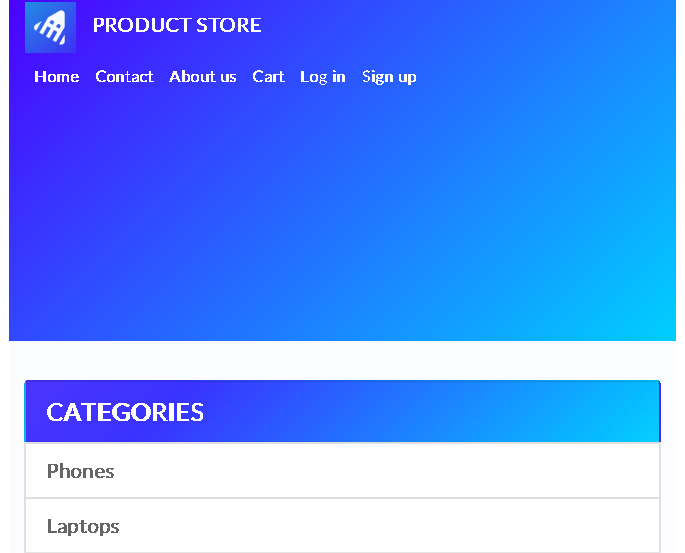
\includegraphics[width=0.6\textwidth]{compat-ios.png}
\caption{Demoblaze en Safari sobre un iPhone real. La tienda carga completa: menú, categorías y productos con sus imágenes.}
\end{figure}

Con esto, los tres motores del mundo quedan probados en escritorio y en móvil. El
resto de combinaciones (versiones antiguas, navegadores marginales) se prioriza
según a quién afecten.

\subsection*{3.13 Cronograma de ejecución}
\addcontentsline{toc}{subsection}{3.13 Cronograma de ejecución}

El cronograma ordena la ejecución. Dejé los bloques cortos a propósito, para que si
el sitio se cae no se pierda mucho trabajo.

\begingroup
\small
\renewcommand{\arraystretch}{1.2}
\begin{table}[htb]\centering\small
\caption{Bloques de ejecución previstos.}\label{tab:crono}
\begin{tabularx}{\textwidth}{@{}L{2.4cm} L{5.4cm} Y@{}}
\toprule
\textbf{Bloque} & \textbf{Actividad} & \textbf{Salida} \\
\midrule
B0, 30 min & Verificación de los criterios de entrada y prueba de sanidad. & Ambiente confirmado o ejecución abortada. \\
B1, 2 h & Los 22 casos de prioridad alta: compra, carrito, autenticación, registro, integración, rendimiento y seguridad. & Criterio S1 cubierto. \\
B2, 2 h & Los 27 casos de prioridad media. & Cobertura por encima del 90\,\%. \\
B3, 45 min & Los 5 casos de prioridad baja y reejecución de los que quedaron bloqueados. Dos de ellos, carga y estrés, quedan marcados como no ejecutables en este entorno. & Suite completa. \\
B4, 1 h & Consolidación de defectos e informe de resumen. & Criterios de salida evaluados. \\
\bottomrule
\end{tabularx}
\end{table}
\endgroup

Si se acaba el tiempo, corto al final de B1. Con los casos de prioridad alta ya
corridos se cumple el criterio S1, y el informe se puede entregar anotando la
cobertura parcial como desviación.

%------------------------------------------------------------------
\FloatBarrier
\section*{4. Entregables}
\phantomsection\addcontentsline{toc}{section}{4. Entregables}

Esta tabla lista lo que sale del proceso de pruebas, con qué lleva cada cosa y en
qué formato. Tres de los seis ya están hechos y van junto con este plan.

\begingroup
\small
\renewcommand{\arraystretch}{1.2}
\begin{center}\small
\captionof{table}{Entregables del proceso de pruebas.}\label{tab:entregables}
\begin{tabularx}{\textwidth}{@{}L{4.2cm} Y@{}}
\toprule
\textbf{Entregable} & \textbf{Contenido y formato} \\
\midrule
Plan de pruebas & Este documento. Formato PDF. \\
Suite de casos de prueba & Hoja de cálculo con una fila por caso: identificador, módulo, prioridad, técnica aplicada, precondiciones, pasos, datos de prueba, resultado esperado y criterio de referencia. Esta última columna materializa lo descrito en el apartado 3.4: cada caso declara contra cuál de los cuatro criterios se juzga el resultado. \\
Registro de ejecución & Identificador del caso, fecha y hora, versión del navegador, resultado (aprobado, fallido, bloqueado, no concluyente) y referencia a la evidencia. \\
Reporte de defectos & Uno por defecto: identificador, título, pasos de reproducción, resultado obtenido contra el esperado, severidad, evidencia y módulo afectado. \\
Evidencias & Capturas de pantalla asociadas a cada caso fallido y a cada defecto. \\
Informe de resumen & Casos diseñados y ejecutados, tasa de aprobación, defectos por severidad y por módulo, desviaciones respecto del plan y conclusión sobre el cumplimiento de los criterios de salida. \\
\bottomrule
\end{tabularx}
\end{center}
\endgroup

Para que se entienda el formato, así queda un caso de la suite:

\begingroup
\small
\renewcommand{\arraystretch}{1.2}
\begin{center}\small
\captionof{table}{Ejemplo de un caso de prueba en el formato definido.}
\begin{tabularx}{\textwidth}{@{}L{3.2cm} Y@{}}
\toprule
Identificador & CP-COM-04 \\
Módulo & Orden de compra \\
Prioridad & Alta \\
Técnica & Tabla de decisión \\
Precondición & Carrito con al menos un producto y ventana de compra abierta. \\
Pasos & 1. Dejar vacíos los campos Nombre y Tarjeta. 2. Completar País y Ciudad con valores válidos. 3. Pulsar Purchase. \\
Resultado esperado & El sistema impide la compra y señala los campos obligatorios sin completar. No se genera comprobante ni se vacía el carrito. \\
\bottomrule
\end{tabularx}
\end{center}
\endgroup

%------------------------------------------------------------------
\FloatBarrier
\section*{5. Dependencias}
\phantomsection\addcontentsline{toc}{section}{5. Dependencias}

\begin{enumerate}[label=D\arabic*.]
  \item \textbf{Que el sitio esté arriba.} Es la dependencia más importante.
        Demoblaze es un servicio gratuito de un tercero, sin acuerdo de nivel de
        servicio y sin ningún compromiso de estar disponible. Si se cae, no puedo
        hacer nada.
  \item \textbf{Estabilidad de los datos de demostración.} Los casos del catálogo
        se apoyan en los productos y categorías existentes. Si el proveedor los
        cambia, hay que actualizar los resultados esperados.
  \item \textbf{Conectividad a internet} desde el equipo de pruebas.
  \item \textbf{Navegador de referencia} en la versión declarada en la sección 6.
  \item \textbf{Que el equipo pueda trabajar.} Al ser solo dos personas, la baja
        de cualquiera reduce a la mitad la capacidad y recarga al otro.
\end{enumerate}

Hay una diferencia con un proyecto normal. Katalon (s.f.)
dice que las dependencias típicas son módulos o servicios que el equipo de
desarrollo todavía no termina, y recomienda dejar módulos simulados para esos casos.
Aquí eso no pasa: el sistema ya está completo y en producción desde antes de que
empezáramos. Todas nuestras dependencias son externas y ninguna la puedo negociar. Eso hace
la planeación más predecible, pero también significa que no puedo hacer nada si
alguna falla.

%------------------------------------------------------------------
\FloatBarrier
\section*{6. Entorno de pruebas}
\phantomsection\addcontentsline{toc}{section}{6. Entorno de pruebas}

\begingroup
\small
\renewcommand{\arraystretch}{1.2}
\begin{table}[htb]\centering\small
\caption{Configuración del entorno de pruebas.}\label{tab:entorno}
\begin{tabularx}{\textwidth}{@{}L{4.2cm} Y@{}}
\toprule
\textbf{Elemento} & \textbf{Configuración} \\
\midrule
Sistema bajo prueba & \url{https://www.demoblaze.com}, entorno de producción del proveedor. \\
Navegador de referencia & Google Chrome. La versión exacta se registra el día de ejecución y se anota en el registro, porque el navegador puede actualizarse solo entre sesiones. \\
Sistema operativo & macOS. \\
Resolución de pantalla & 1920 por 1080, con una verificación adicional a 1366 por 768 para el comportamiento responsivo básico. \\
Datos de prueba & Usuario y contraseña ficticios creados para el ejercicio, número de tarjeta ficticio, y valores de borde por campo. No se emplean datos personales reales. \\
Herramientas & Navegador con sus herramientas de desarrollo para inspeccionar la interfaz, y captura de pantalla para la evidencia. \\
Accesos no disponibles & Código fuente, servidor, base de datos, registros de aplicación y consola de administración. \\
\bottomrule
\end{tabularx}
\end{table}
\endgroup

La diferencia grande con un plan normal es que no hay un ambiente de pruebas aparte.
Pruebo directamente sobre la producción del proveedor, la misma que está usando
cualquier otra persona en ese momento. De ahí salen dos cosas que afectan todo el
plan: no puedo hacer pruebas destructivas ni de carga, y los datos pueden cambiar de
una sesión a otra porque alguien más los tocó. Las dos quedan anotadas en la sección
siguiente, donde separo lo que son restricciones de lo que son riesgos de verdad.

%------------------------------------------------------------------
\FloatBarrier
\section*{7. Gestión de riesgos}
\phantomsection\addcontentsline{toc}{section}{7. Gestión de riesgos}

\subsection*{7.1 Clasificación de severidad de defectos}
\addcontentsline{toc}{subsection}{7.1 Clasificación de severidad de defectos}

Uso la clasificación del documento de ejemplo que venía con el taller, ajustada a
este sitio:

\begin{itemize}
  \item \textbf{Crítico}: impide completar el flujo de compra, muestra información
        errónea de precios o totales, o expone funciones que deberían requerir
        sesión iniciada.
  \item \textbf{Medio}: falla una función secundaria, o una validación no impide
        una entrada claramente inválida sin llegar a bloquear la compra.
  \item \textbf{Leve}: defectos de presentación, textos, coherencia visual o
        comportamientos distintos ante situaciones equivalentes.
\end{itemize}

\subsection*{7.2 Restricciones asumidas, que no son riesgos}
\addcontentsline{toc}{subsection}{7.2 Restricciones asumidas, que no son riesgos}

Hay tres condiciones de este ejercicio que ya sabía antes de escribir el plan, así
que su probabilidad es del 100 por ciento. No son riesgos, porque un riesgo es algo
incierto que se puede gestionar. Son restricciones y se asumen. Las separo para no
llenar la tabla de riesgos con cosas que no lo son.

\begin{enumerate}[label=C\arabic*.]
  \item \textbf{No hay ambiente de pruebas separado.} Se trabaja sobre la
        producción compartida del proveedor. De ahí la prohibición de pruebas de
        carga, estrés e intrusivas, y el uso exclusivo de datos ficticios.
  \item \textbf{Los defectos encontrados no se pueden corregir.} El objetivo se
        redefine hacia documentar y evaluar impacto en lugar de certificar, según
        el apartado 2.3.
  \item \textbf{La ejecución se hace en una sola ventana de trabajo.} De ahí la
        priorización del apartado 3.6 y el criterio de salida S1, que exige el
        100\,\% de los casos de prioridad alta y no del total.
\end{enumerate}

\subsection*{7.3 Riesgos identificados}
\addcontentsline{toc}{subsection}{7.3 Riesgos identificados}

\begingroup
\footnotesize
\setlength{\tabcolsep}{4pt}
\renewcommand{\arraystretch}{1.2}
\begin{center}\footnotesize
\begin{minipage}{\textwidth}
\captionof{table}{Riesgos del proceso de pruebas y su mitigación.}
\begin{tabularx}{\textwidth}{@{}L{0.9cm} Y L{1.5cm} L{1.5cm} Y@{}}
\toprule
\textbf{Cód.} & \textbf{Riesgo} & \textbf{Probab.} & \textbf{Impacto} & \textbf{Mitigación} \\
\midrule
R1 & El sitio queda fuera de servicio durante la ejecución. & Media & Alto & Ejecutar en los bloques cortos del apartado 3.13 y capturar la evidencia de cada caso en el momento, sin dejarla para el final. \\
R2 & El proveedor cambia el sitio o reinicia los datos a mitad del trabajo. & Media & Medio & Diseñar casos independientes entre sí, cada uno con su propia precondición. Reejecutar la suite de regresión si se detecta un cambio. \\
R3 & El mismo equipo que diseña los casos los ejecuta, con riesgo de sesgo de confirmación. & Media & Medio & Que una persona diseñe cada caso y la otra lo revise y ejecute, para que el diseño y la ejecución no recaigan en la misma persona. \\
R4 & El criterio de referencia elegido no corresponde al caso y se reporta como defecto un comportamiento correcto. & Media & Medio & Declarar el criterio en la columna respectiva de la suite, de modo que la decisión quede auditable y se pueda revisar si alguien discrepa. \\
R5 & La evidencia capturada no permite reproducir el defecto después. & Media & Medio & Capturar la pantalla completa con la URL visible y anotar los datos exactos de entrada en el registro de ejecución. \\
R6 & El sitio usa diálogos de JavaScript para confirmar acciones, lo que bloquea la automatización. & Media & Bajo & Ejecución manual en esta iteración. Evaluar el manejo de diálogos antes de automatizar. \\
\bottomrule
\end{tabularx}
\end{minipage}
\end{center}
\endgroup

R3 es el mismo problema de independencia que aparece cuando un equipo prueba lo que
él mismo construyó. Con solo dos personas no se puede eliminar, pero sí atenuar
haciendo que quien diseña un caso no sea quien lo ejecuta, como indica la mitigación de la tabla.

\section*{8. Roles y responsabilidades}
\phantomsection\addcontentsline{toc}{section}{8. Roles y responsabilidades}

Los roles se organizan por función, indicando quién asume cada una. Al ser un
equipo de dos, cada integrante concentra varias responsabilidades, pero el diseño
de los casos y su ejecución se asignan a personas distintas a propósito, por lo que
se explica debajo de la tabla.

\begingroup
\small
\renewcommand{\arraystretch}{1.2}
\begin{center}\small
\captionof{table}{Roles, responsabilidades y asignación.}
\begin{tabularx}{\textwidth}{@{}L{3.4cm} Y L{3.2cm}@{}}
\toprule
\textbf{Rol} & \textbf{Responsabilidad} & \textbf{Asignado a} \\
\midrule
Líder de pruebas & Definir alcance, estrategia y criterios de entrada y salida. Aprobar el cierre de la actividad. & Joshua Mendez \\
Diseñador de casos & Derivar los casos de prueba aplicando las técnicas de la sección 3 y documentar el resultado esperado de cada uno. & Joshua Mendez \\
Ejecutor de pruebas & Ejecutar los casos, registrar resultados y recolectar evidencia. & Edinson Pedroza \\
Gestor de defectos & Registrar y clasificar los defectos, evaluar su impacto y redactar el informe de resumen. & Edinson Pedroza \\
Aprobador & Revisar el plan y el informe final, y dar por recibida la entrega. & Claudia Martínez, docente del curso \\
\bottomrule
\end{tabularx}
\end{center}
\endgroup

El reparto separa a propósito el diseño de la ejecución: Joshua Mendez diseña los
casos y Edinson Pedroza los ejecuta. Así atacamos el riesgo R3 de la sección
anterior, porque el sesgo de confirmación pega más fuerte cuando quien escribió un
caso es quien lo ejecuta —tiende a correrlo esperando que salga como lo pensó—. Con
dos personas no se elimina del todo (ambos redactamos el plan y revisamos el
trabajo), pero sí se reduce al no concentrar diseño y ejecución en la misma mano.

%------------------------------------------------------------------
\FloatBarrier
\section*{Referencias}
\phantomsection\addcontentsline{toc}{section}{Referencias}

\begingroup
\setlength{\parindent}{-1.6em}
\setlength{\leftskip}{1.6em}
\setlength{\parskip}{7pt}

Google. (2024). \emph{Web Vitals: umbrales de las métricas web esenciales}.
https://web.dev/articles/vitals

International Organization for Standardization. (2011). \emph{ISO/IEC 25010:2011.
Systems and software engineering. Systems and software Quality Requirements and
Evaluation (SQuaRE). System and software quality models}. ISO.

International Software Testing Qualifications Board. (2018). \emph{Certified Tester
Foundation Level syllabus} (cap. 2). ISTQB.

Katalon. (s.f.). \emph{Test plan vs. test strategy: key distinctions and
components}. \url{https://katalon.com/resources-center/blog/test-plan}

Martínez, C. (2026a). \emph{Niveles de pruebas} [Diapositivas]. Construcción de
Software y Pruebas, Pontificia Universidad Javeriana.

Martínez, C. (2026b). \emph{Tipos de prueba} [Diapositivas]. Construcción de
Software y Pruebas, Pontificia Universidad Javeriana.

World Wide Web Consortium. (2018). \emph{Web Content Accessibility Guidelines
(WCAG) 2.1}. W3C. https://www.w3.org/TR/WCAG21/

\endgroup

\end{document}
